\chapter{Costing}
\label{chap:costing}
%\writer{Henri Videau}{6}
%\section{Introduction}
This chapter presents an updated costing of the ILD detector, corresponding to its latest baseline design and dimensions as used in the simulations for performance evaluation. The method is very similar to that used in the costing exercise of the DBD, with two notable differences. Two size options are now costed: the large model IDR-L, very similar to the DBD baseline, and the small model IDR-S where the outer radius of the TPC has been reduced by about 30cm. In addition, the required manpower is now included in the costs, in an attempt to identify the in-kind laboratory manpower necessary to assemble the detector. 

The costing can now benefit from the construction of significant technological prototypes of the main subdetectors (chapter 5), as well as from spin-off detectors starting to be built for e.g. HL-LHC. The cost difference of the two models combined with the differences observed in their respective performances (chapter 8) will allow a better evaluation of the impact of the detector size than the simple scaling laws shown in the DBD. 

\section{The method}
The DBD costing had been made in an "ILC currency", the ILCU, in an effort to have a costing coherent between ILD, SiD and the accelerator. This implied making translations from different currencies using exchange rates and, in most cases, "Purchase Power Parities" (PPP). At that time an ILCU was 0.97 Euros using PPP's. Within the current exercise Euros(2018) are used as currency unit. When originating from Japan, e.g. for silicon diode matrices, prices in Euros were provided by the vendors. Extrapolation of the DBD estimates to the present is made by converting the DBD ILCU's to Euros(2013) using PPP's as was done at that time (0.97 Euros for 1 ILCU), and propagating the cost to 2018 using as inflation rate the evolution of manufactured products in Europe, amounting to 3\% between 2013 and 2018, as shown in figure~\ref{price_index}. The two factors compensate and 1 DBD ILCU turns out to be equivalent to 1 Euro(2018). 
%(\textit{figure Berriaud}).

\begin{figure}[h!]
\centering
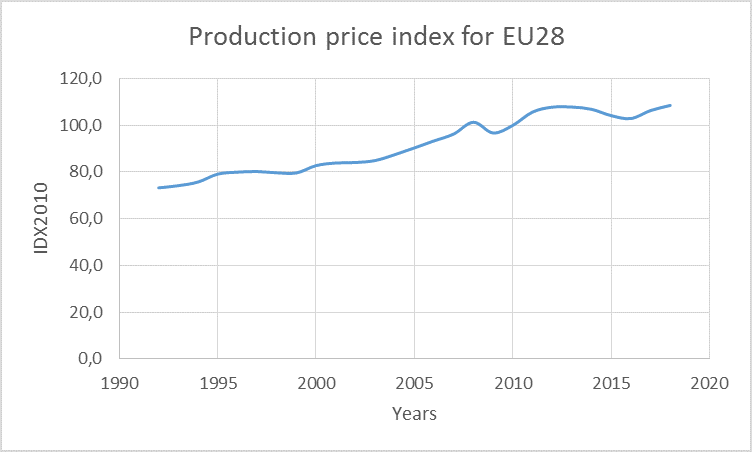
\includegraphics[width=1.0\hsize]{Costing/price_index.png}
\caption{Manufactured products price evolution over the 28 countries of UE.}
\label{price_index}
\end{figure}

Except for the currency, the method used to establish the costing is totally similar to that of the DBD. It rests on the detailed knowledge of the fabrication processes and on the prices provided by the numerous prototypes built over the past years.  The idea is to identify the cost drivers, often very sensitive to strong price evolution, and to have a precise Work Breakdown System (WBS) identifying the procurements, the tooling and the fabrication operations. The WBS allows to estimate the manpower, which is now included in the costing. The manpower is twofold: in house laboratory  manpower mostly linked to the follow-up of the operations, but also to some construction work when high quality is required for small quantity items; industrial manpower which has to be estimated on top of the material costs in case no industrial offer is available for a given component. The manpower costs are converted into Euros(2018) assuming 80k\texteuro~per FTExYear as a mean unit cost over the different types of competences. The industrial manpower is incorporated into the material costs, whereas the in house manpower is shown separately as an estimation of the in-kind contributions of the participating institutes. 
It should be noticed that spares are most of the time not included. More generally no contingency is applied.

\section{Subdetector costing}
The cost of each ILD subdetector is reviewed for the IDR-L and IDR-S models. The inner and forward detectors which have the same configuration in both options (VTX, SIT, FTD, ECAL ring, LumiCAL, LHCAL, BeamCAL) have only one quote, whereas others (TPC, ECAL, HCAL, Coil, Yoke and Iron Instrumentation) are costed for their two size versions. The subdetector baseline costing is made for the layouts described in section 5.1.2 and used in the performance evaluations of chapter 8. In some cases a costing is also estimated for modified or upgraded designs corresponding to the ongoing studies reported in section 5.2.   

The most expensive subdetector, the SiECAL, has received special attention in updating its costing of both material and manpower contributions, based on an updated detailed WBS. Some other subdetectors have fewer new pieces of information. For those which have only material costs available, the manpower costing has been estimated assuming the same manpower/material ratio as for the SiECAL. When no update is available w.r.t the DBD version, the costing is propagated from the DBD estimate and simple scaling laws are used for the small version.

In the following, when a cost estimate appears as two numbers inside brackets, the first number corresponds to the material cost and the second one to the in house manpower.

\subsection{VTX}
The Vertex Detector costing has been fully revisited %[ref \textit{Note "ILD VXD and SIT Costing Estimates" by Marc Winter and Auguste Besson June 2019}] 
for its CMOS option based on recent detectors built for various experimental projects (see section 5.2.1). The results are summarised in  table~\ref{vertex_cost}. The cost for this option is (2.96, 1.45) M\texteuro. A DEPFET option has also been reexamined leading to a similar cost of (3.44, 1.5) M\texteuro.

%\textit{Mention also note of DEPFET estimation for VTX and FTD }

%\textit{Check that manpower corresponds to in house only, in view of the size it is very likely}

\begin{table}\hspace*{-0cm}\small
\begin{tabular}[h!]{ l p{0.1\hsize}p{0.1\hsize}p{0.1\hsize} p{0.1\hsize}p{0.1\hsize}p{0.1\hsize} }
\toprule
\multicolumn{7}{ l }{{\bf Vertex detector}}\\
\midrule
Cost   & Sensors & Mechanics & Electronics & Services & Installation & Total \\
\midrule
Material    & 1.15   &  0.45   &  0.49    & 0.77 & 0.10 & 2.960 \\
Manpower    & 0.10   & 0.50    & 0.40     & 0.25 & 0.20 & 1.450 \\
\midrule
Total      & 1.25   &  0.95   &  0.89    & 1.02 & 0.30 & 4.410 \\
 \bottomrule
\end{tabular}
\caption{\label{vertex_cost}Elements of cost of the vertex detector (CMOS option) in M\texteuro.}
\end{table}

%\begin{figure}[h!]
%\centering
%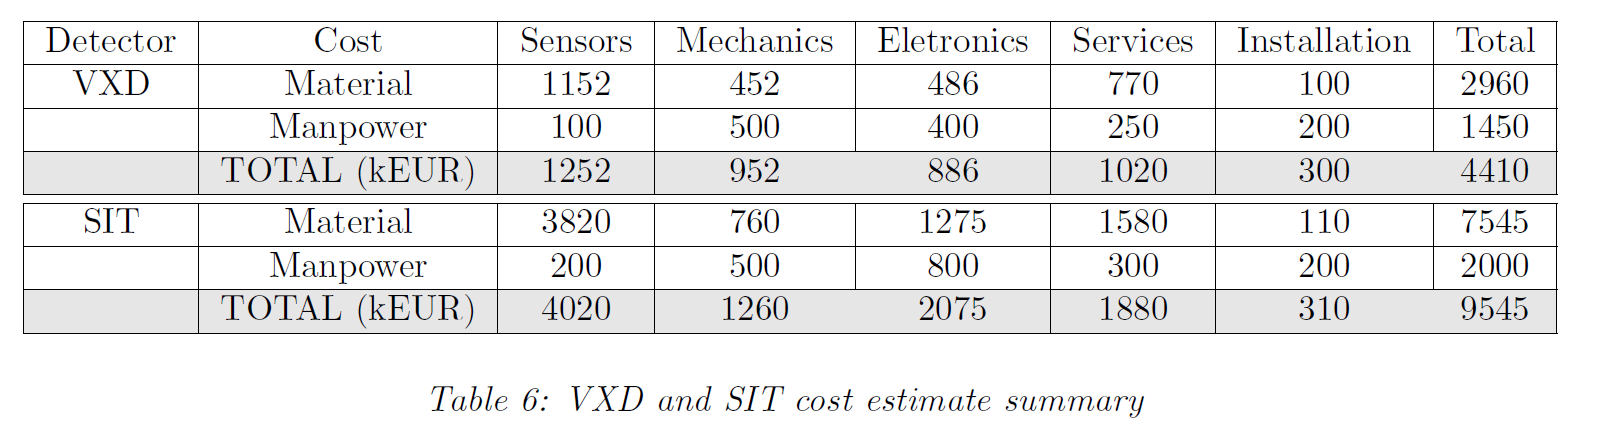
\includegraphics[width=1.0\hsize]{Costing/VXD_SIT.PNG}
%\caption{Contributions of the different items to the cost of the vertex detector.}
%\label{VXD_SIT}
%\end{figure}

\subsection{SIT}
In its baseline design used for estimating the physics potential of the detector, the SIT is made of strips as in the DBD. The cost of this strip version could be estimated similarly to the SET (see later), using an areal extrapolation from the CMS tracker tempered by a reasonable account of items which do not scale with surface. This extrapolation is well compatible with the costs of the smaller silicon strip beam telescope LYCORIS recently built for the DESY TPC test setup (section 5.2.3). The resulting estimated cost of the baseline strip version of the SIT is (5, 1.5)M\texteuro.

The SIT costing has also been revisited in detail in a version based on CMOS pixels. The inputs are the same as used for the VTX CMOS costing,  
%[ref \textit{Note "ILD VXD and SIT Costing Estimates" by Marc Winter and Auguste Besson June 2019}]
and the results summarised in table~\ref{SIT_cost}. It can be observed that the total cost of (7.55, 2) M\texteuro~ of the pixel SIT does not scale with the area compared with the VTX: the cost factor is about 3 for an area factor of about 20.
%It can be noted that the pixel option appears more expensive than the strip option.

%\textit{Check that manpower corresponds to in house only} sit area 1.53 m²


\begin{table}\hspace*{-0cm}\small 
\begin{tabular}[h!]{ l p{0.1\hsize}p{0.1\hsize}p{0.1\hsize} p{0.1\hsize}p{0.1\hsize}p{0.1\hsize} }
\toprule
\multicolumn{7}{ l }{{\bf Silicon Inner Tracking}}\\
\midrule
Cost   & Sensors & Mechanics & Electronics & Services & Installation & Total \\
\midrule
Material    & 3.82   &  0.76   & 1.28    & 1.58 & 0.11 & 7.55 \\
Manpower    & 0.20   & 0.50    & 0.80    & 0.30 & 0.20 & 2.00 \\
\midrule
Total      & 4.02   &  1.26   &  2.08    & 1.88 & 0.31 & 9.55 \\
\bottomrule
\end{tabular}
\caption{\label{SIT_cost}Elements of cost of the SIT (CMOS pixel option) in M\texteuro.}
\end{table}

\subsection{FTD}
There is no full update since the DBD. The current FTD baseline configuration (chapter 5) includes 4 disks using pixel technology and 10 disks using strip technology. The cost of the sole 4 pixel disks in the CMOS version is estimated to (1.1, 0.2) M\texteuro, whereas an option using DEPFET has been estimated to (2.05, 1.5) M\texteuro.
The cost of the strip disks is inferred to be (3.7, 1.1) M\texteuro~ similarly as for the strip SIT. The global cost for the baseline option is then of the order of (4.8, 1.3) M\texteuro. 

A direct comparison to the DBD estimate is possible only at the level of the global inner silicon tracking (SIT + FTD). The DBD was quoting 2.3 M\texteuro~ without manpower when the new estimate is (9.8, 2.8) M\texteuro.

The cost of a fully pixelised FTD made of 14 disks with CMOS pixels was estimated similarly to the pixel SIT case to (9.1, 1.7) M\texteuro.
%was 12.3, 3.3   MDIFIER LES TABLES. ,????
%règle de somme: FTD  + SIT (2.2, 0.5) + (1.0, 0.1) comparés au DBD  2.3 ME%\textit{Mention and take into account DEPFET estimation note}
% normalisation SET (16, 2) pour 53m² soit  (0.306, 0,038) per m²
% aires des disques: pixels 0.3 m² , strips 2.22, total 2.52   total over pixels = 8.4
%?du SET 0.25+0.04 du m². Soit strips 0.56 + 0.09
% La surface du SIT est 3.06     soit 0.94 + 0.12  en strips        et (7.55, 2.)    en pixels
% disques strips 2.22m² soit (O.68, 0.084) si SIT (5, 1.5) les disques strips  font 

%disques pixel 0.3 m²  1.47 + 0.4     should be 1/2
% donc modele classique 2.03 + 0.5
%modele pixel = (7.55, 2.) 3.06 / 2.52 * = (6.2, 1.65)  was 12.3 +3.3 a factor 2??

It has to be noted that the cost of the structure (called ISS) holding the beam tube, the vertex detector, the SIT and the FTD has not been estimated.

\subsection{Forward Calorimetry (FCAL)}

Three forward calorimeters, namely the BeamCAL, the LumiCAL and the LHCAL, have been reexamined in detail in their new configuration with the new beam optics (chapter 5). The updated costing includes consideration of the mechanical elements, sensors, ASICs, front-end electronics, power supplies, data acquisition, tooling and manpower, separately for each of the subdetectors. Ancillary systems such as specific fanouts (for LumiCAL and LHCAL) and a laser positioning system needed for LumiCAL are also included. The resulting costs are summarised in table~\ref{FCals_summary}. They correspond to a total of 8.44 M\texteuro~ and 6 FTExYears equivalent to 0.48M\texteuro.

%\textit{Trivial question: the costing is summing the 2 systems in both beam directions ?} 

The forward region also includes an ECAL ring making the transition from the LumiCAL to the ECAL endcap. Its costing has been updated based on a rough silicon area extrapolation from the SiECAL costing (see below). The ECAL rings silicon area is about  1\% of the full SiECAL, barrel plus end-caps. The electronics is more similar to that of the LumiCAL and the manpower is taken identical to that needed for the LumiCAL.  The estimated cost of the two rings is then (1.5, 0.16) M\texteuro.  

The whole forward calorimetry, including BeamCAL, LumiCAL, LHCAL and ECAL ring, and referred to as FCAL in Figures ~\ref{fig:det:DBD_cost_sharing} and ~\ref{Costing:Small_cost_sharing}, is then estimated to (10, 0.6) M\texteuro. The cantilevered beam structure holding the QD0 focussing quadrupoles but also the forward calorimetry has not been costed in the detector part.

%\begin{figure}[h!]
%\centering
%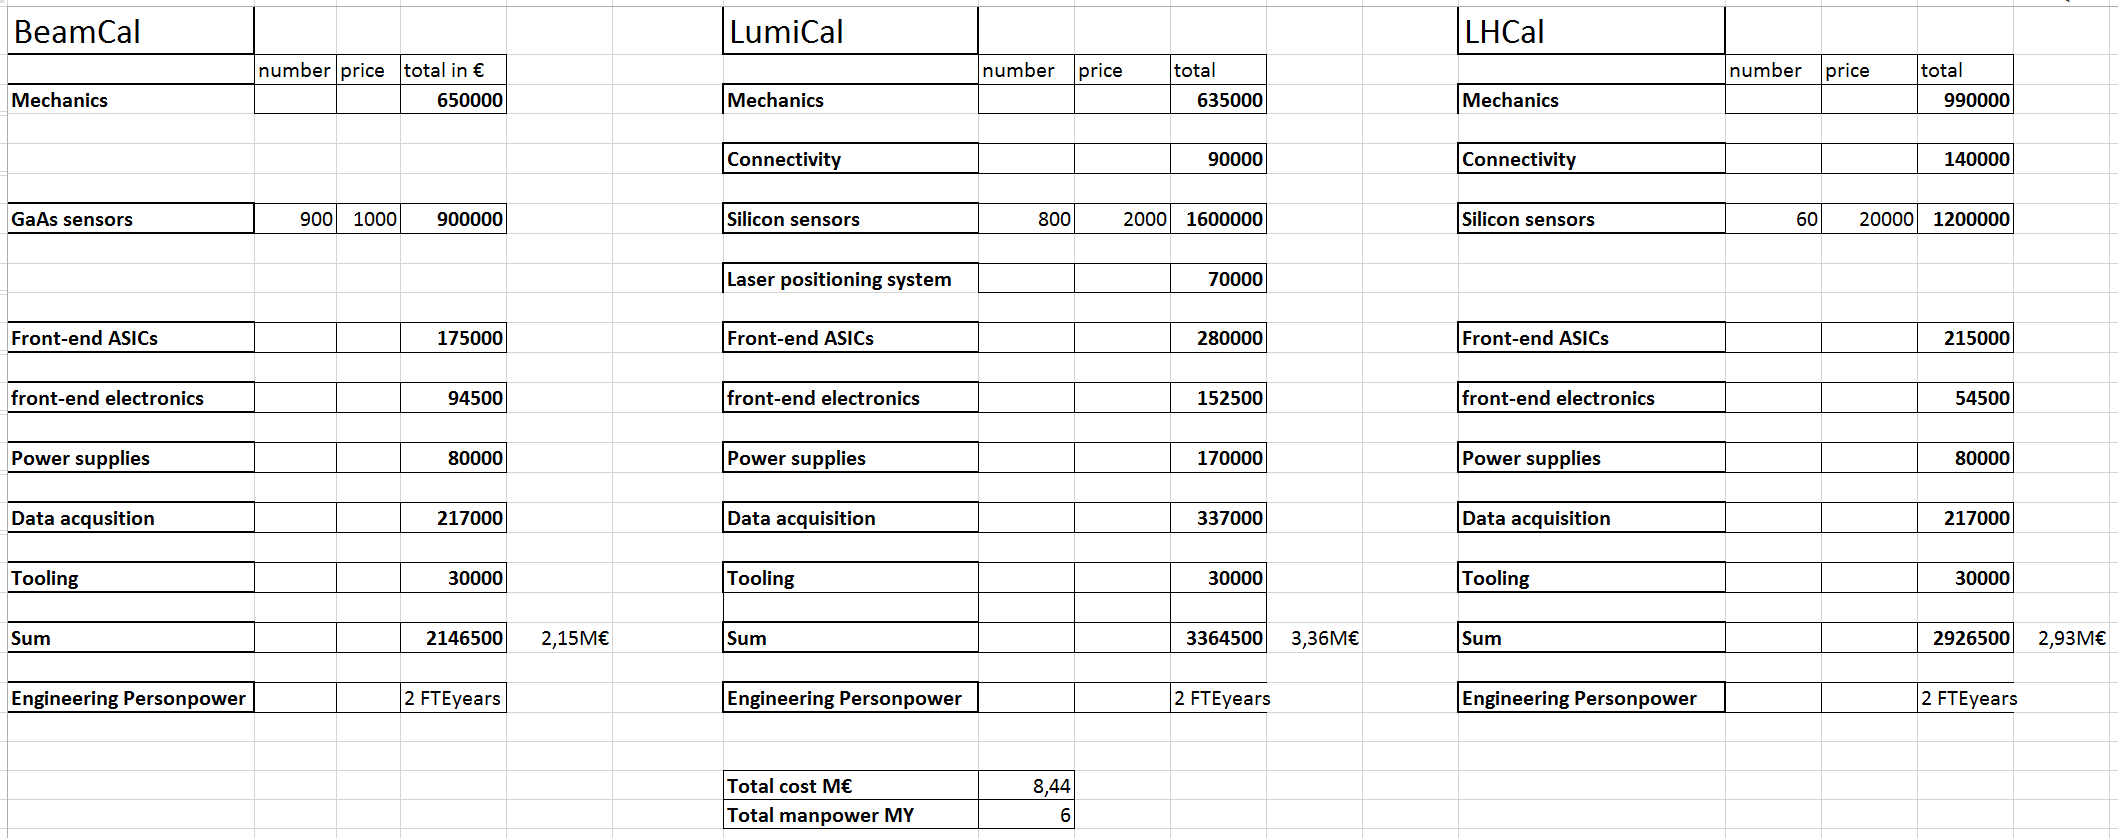
\includegraphics[width=1.\hsize]{Costing/Fcals_summary.PNG}
%\caption{Contributions of the different items to the cost of the forward calorimetry.}
%\label{Fcals_summary}
%\end{figure}

 \begin{table}\hspace*{-0cm}\small 
\begin{tabular}[h!]{ l p{0.2\hsize}p{0.2\hsize}p{0.2\hsize} }
\toprule
& BeamCAL & LumiCAL & LHCAL \\
\midrule
Mechanics              & 0.65   & 0.64   & 0.99   \\
Connectivity           &        & 0.09   & 0.14   \\
Sensors                & 0.90   & 1.60   & 1.20  \\
Laser system           &        & 0.07   &       \\
Front-end ASICs        & 0.18   & 0.28   & 0.22   \\
Front-end electronics  & 0.10   & 0.15   & 0.05  \\
Power supplies         & 0.08   & 0.17   & 0.08    \\
Data acquisition       & 0.22   & 0.34   & 0.22  \\
Tooling                & 0.03   & 0.03   & 0.03   \\
\midrule
Total                  & 2.15  & 3.37   & 2.93  \\
\midrule
Manpower (FTE x Year)  &2       &2       & 2 \\
\bottomrule
\end{tabular}
\caption{\label{FCals_summary}Elements of cost of the forward calorimeters in M\texteuro~ and manpower in FTE x Year.}
\end{table}

\subsection{TPC}
The quoted TPC price of the DBD corresponds to 36 M\texteuro(2018) including $\approx$5 M\texteuro~ of manpower. The TPC dimensions  were very close to those of today's large IDR-L option of ILD.
%No specific in-house manpower had been estimated.

%Recently one of the options for the TPC has been costed again with many more details. This cost has been estimated for the option using Micromegas detectors. The cost is derived from the cost of the TPC built in that technology for the T2K experiment.

Since then two TPC projects with similar technologies are progressing towards construction : ALICE with GEM readout, and T2K/ND280 High Angle with resistive anode Micromegas readout. The T2K/ND280 project has allowed to update the TPC costing in the Micromegas option with many details, including manpower and taking into account requirements imposed by Japanese regulations. Similarly the ALICE project has allowed an update for the GEM option. The construction of a new field cage for the DESY TPC test setup (section 5.2.3) has also strongly modified the estimate of the field cage cost. The costs can be split into a technology-independent part and a technology-dependent part.

%The technology independent part comprises the electrostatic system for 5.8 ME (including test and shipping), the ancillaries for 2.7 ME (CO2 compressor, TPC gas system, laser system, power supplies, their packing and shipping) and the overall management for 1.2 ME. The total technology independent cost estimate is therefore (8.5, 1.2) ME.
The technology-independent part comprises the electrostatic system for 1.8 M\texteuro~ (including test and shipping), the TPC hanging system for 0.2 M\texteuro~, the ancillaries for 2.7 M\texteuro~ (CO2 compressor, TPC gas system, laser system, power supplies, their packing and shipping) and the overall management for 1.2 M\texteuro. The total technology-independent cost estimate is therefore (4.8, 1.1) M\texteuro.

%The technology dependent part consists of everything which is sensitive to the pad size and the module size. It includes the end plates, the readout modules, the electronics, the cables and pipes as well as the assembly. In the micromegas option its costing is currently estimated to (14.5, 5) ME. The lower cost compared to DBD is mainly related to the mechanical costs of the endplates and readout modules, and to accounting for prototyping in the DBD estimation.
The technology-dependent part consists of everything which is sensitive to the pad size and the module size. It includes the end plates, the readout modules, the electronics, the cables and pipes as well as the assembly. The manpower is estimated to be equal in the two solutions. The Micromegas option costing is currently estimated to (11.6, 3.9) M\texteuro, whereas the GEM option amounts to (20.4, 3.9) M\texteuro.

%The updated estimate of the total TPC cost in the micromegas option is therefore (23, 6.2) ME, to be compared to (31, 5) ME from the DBD. In order to account for remaining uncertainties associated to the readout technologies and TPC integration, the DBD estimation is conservatively kept as the baseline estimate of the TPC cost. The (31, 5) IDR-L estimate is scaled down to (23.4, 3.6) for the IDR-S version.
The updated estimate of the total TPC cost is therefore (16.4, 5) M\texteuro~ in the Micromegas option and (25.2, 5) M\texteuro~ in the GEM option. 
The largest estimate of (25.2, 5) M\texteuro~ is conservatively kept as the baseline cost. The IDR-L estimate is scaled down to (19, 3.6) M\texteuro~ for the IDR-S version.
%scaling by 0.75
%\textit{ A proper estimate for the GEM version remains to be established. Currently the GEM electronics has been estimated to 25 MEuros difficult to accommodate in the 31 MEuros.}
%\textit{ Any chance to get an update from Paul Colas?}
%\textit{What about manpower ?}

\subsection{SET}
For the DBD the external silicon tracker, SET and ETD, was costed globally. The endcap part, the ETD, is no longer part of the ILD design. Considering that the cost should be roughly proportional to the detector area and that the number of silicon layers was three in the ETD and only two in the SET, the  cost of the SET can be inferred from the DBD to be around 13.4 M\texteuro~(2018) manpower excluded.
%The cost from the DBD is quoted 21 MILCU (MEuro) for SET plus ETD. A cost for the SET alone can be guessed from the areas but the number of layers is different, 3 in the ETD and only 2 in the SET; the SET sensitive area over the total is about 0.64 (0.73), we use this number (SLIGHTLY UNDERESTIMATED) for scaling and its cost is then claimed to be 13.4 MEuros 2008. No cost was established for the small model. It could be scaled from the large with the ratio of the radii: 0.807, providing a cost of 10.8 MEuros.

An estimate of the barrel part (SET) can now be more accurately derived from the cost of the CMS tracker which is also made of double-layer silicon strips. The CMS tracker has a total instrumented area of 220 $m^2$, with a cost of about 275kCHF per $m^2$ of detector, including silicon sensors, front-end electronics, cooling and cabling as well as mechanics. The ancillaries like back-end electronics, cooling plant and power supplies account for 16MCHF globally. This can be considered  as 73kCHF per $m^2$ which add to the 275 to give 306 k\texteuro~ per $m^2$.
The SET area in the IDR-L ILD model is about 52.9 $m^2$. Using the CMS areal cost results in a value of about 16 M\texteuro~which, taking into account items which do not scale with surface, can be converted into a conservative SET material cost estimate of 20 M\texteuro. The in house manpower is estimated to 2 M\texteuro~ providing a total of 22 M\texteuro.
Using a simple scaling law the IDR-S SET is then estimated to (16, 1.5) M\texteuro~ for an area of 42.7 $m^2$. 
%from CMS 275kCHF per $m^2$ of detector, for the 220 m² it gives 60.5 MCHF, which includes silicon sensors, front-end, cabling and cooling and mechanics (modules 3MCHF and structures 6.5). The detector without ancillaries amounts then to 51MCHF for 220m² or 2 200 000 cm², the  detector price per cm² is therefore 27.5 CHF/cm² or 25 Euros.
% Globally the back-end electronics amounts to 6MCHF, cooling plant 6MCHF, power supplies 4MCHF. All this for the 220 m2. It gives 16M for 220 m² equivalent to 73kCHF or 66kE per m². What about the construction cost? 30.6 E/cm², 306kE /m². (16.2, 1.8)

\subsection{ECAL}
\subsubsection{Silicon option of the ECAL (SiECAL)}
The DBD SiECAL costing corresponded to 157 M\texteuro(2018) excluding manpower, with about half of the cost due to the silicon diode matrices.

The updated costing of the SiECAL is based on a very detailed WBS informed from the fabrication processes of the SiECAL technological prototypes (chapter 5). This WBS follows a detailed and chronological fabrication description with the procurements for the different operations, the needed tooling and the fabrication steps, including manpower and duration, under the constraint that none should have a duration longer than two years. Most of the tooling has been kept at the same cost for the different ILD size options, which is slightly at the advantage of the large model for comparison of the costings between the different sizes.

Apart for a slight tungsten cost rise, the main difference with the DBD estimate comes from the evolution of the diode matrices estimation. In the updated costing the offer to CMS for the HGCAL matrices is used. The resulting total SiECAL cost reaches 119 M\texteuro~ excluding manpower. The in house manpower has also been estimated to 131 FTExYears, equivalent to 11 M\texteuro, which results in a total amount of 130 M\texteuro. It should be noted that possible future improvements such as a high timing resolution have not been taken into consideration for this costing.

Using similar inputs the small SiECAL version is costed to 92 M\texteuro~ for material. Including 9 M\texteuro~ for manpower, the total cost is 101 M\texteuro. 
A version of the small SiECAL with a slightly coarser sampling has also been estimated. For this version the number of active layers is reduced from 30 to 26 (section 5.2.4.1). The motivation for such a configuration is dictated by technical reasons rather than cost, but it is worth noting that the impact of the reduced sampling on the energy resolution is expected to be compensated by an increase of the silicon thickness to 725 micrometers. The reduced sampling provides a further cost reduction to (81, 8) M\texteuro.  

The various global costings are summarised in table~\ref{ECal_summary}. A breakdown of the contributions of the main items to the cost is shown in Figure~\ref{fig:det:ECal_Si_cost_sharings} for the three models. The silicon matrices cost still dominates the procurement, but other items such as tungsten, printed boards and ASICs also represent significant parts. The in-house manpower is around 10\% of the cost.

\begin{table}\hspace*{-0cm}\small 
\begin{tabular}[h!]{ l p{0.2\hsize}p{0.2\hsize}p{0.2\hsize} }
\toprule
Version& Material & Manpower & Total \\
\midrule
IDR-L                       & 119   & 11    & 130   \\
IDR-S                       & 92    &  9    & 101   \\
IDR-S with reduced sampling & 81.   &  8    & 89  \\
\bottomrule
\end{tabular}
\caption{\label{ECal_summary}Estimates for the three versions of the SiECAL (M\texteuro).}
\end{table}

\begin{figure}[h!]
\begin{tabular}{ccc}
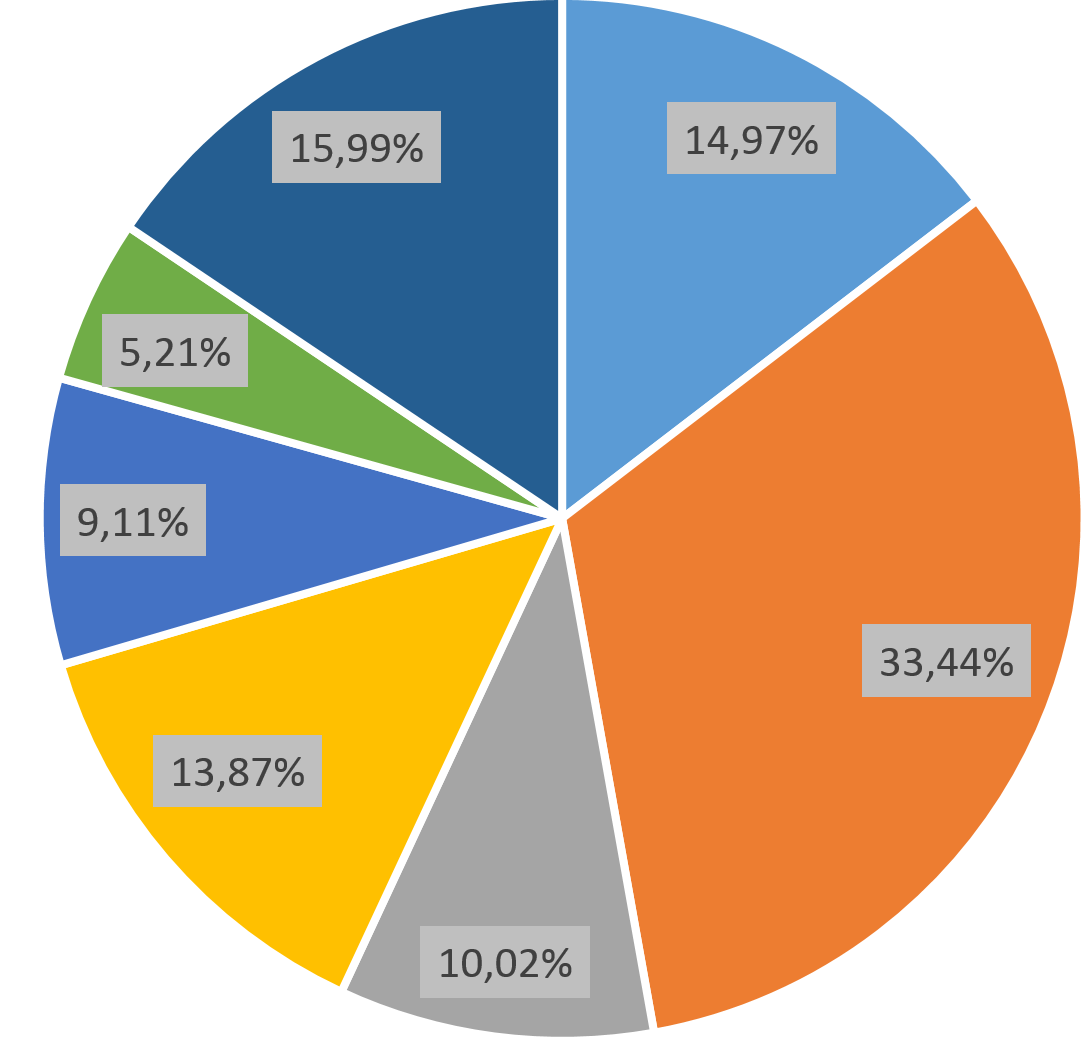
\includegraphics[width=0.3\hsize]{Costing/Eclg_sharing.PNG}&
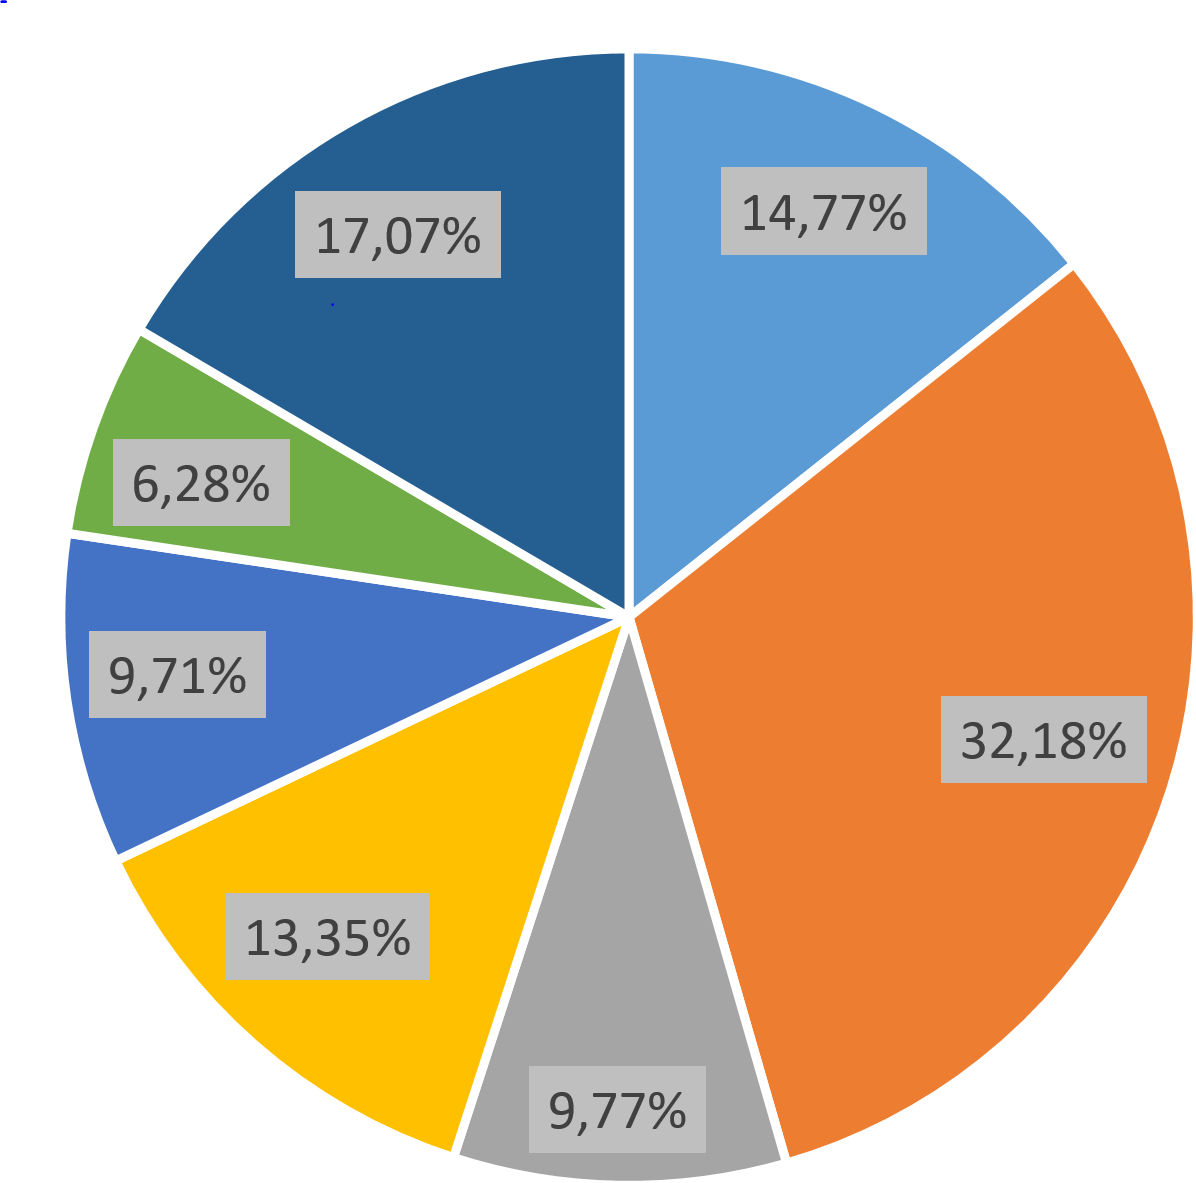
\includegraphics[width=0.3\hsize]{Costing/Ecsm_sharing.PNG}&
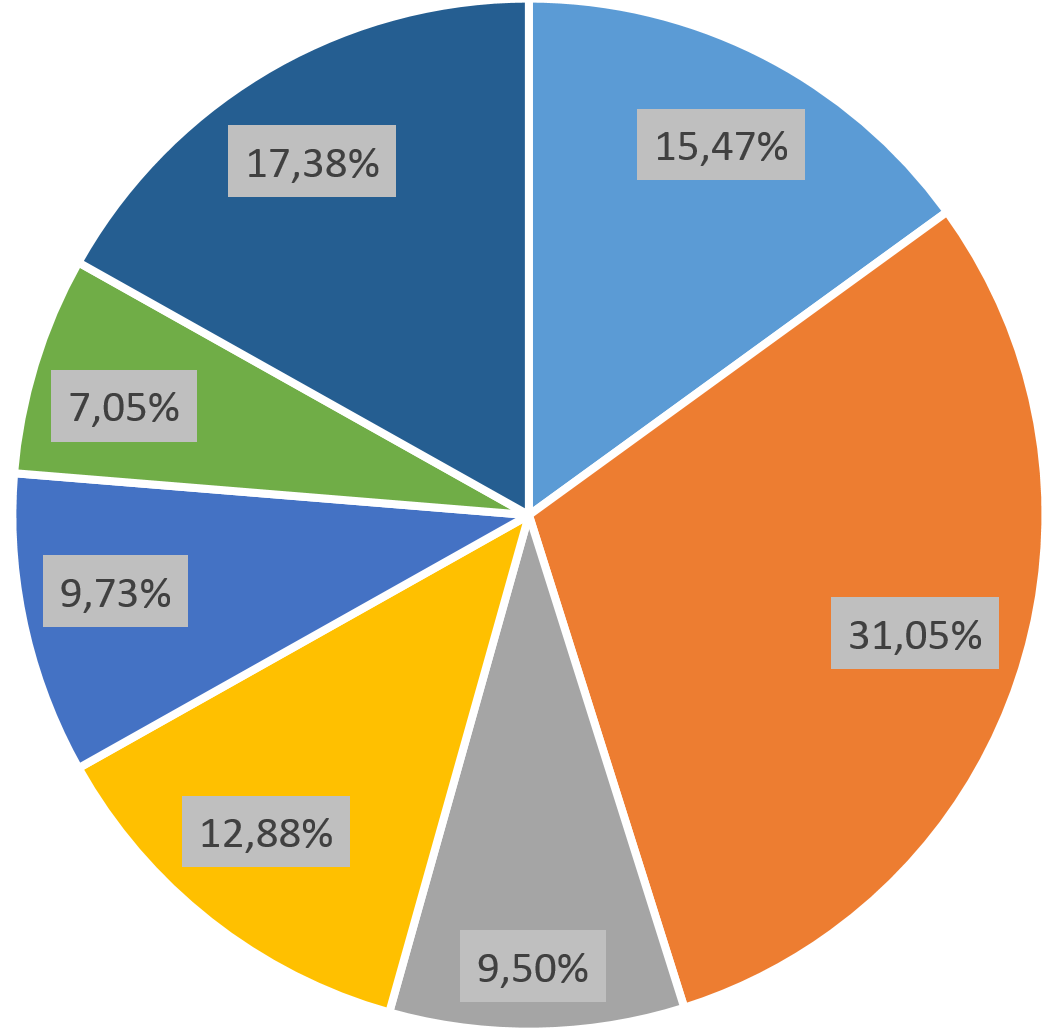
\includegraphics[width=0.3\hsize]{Costing/Ec26_sharing.PNG}
\end{tabular}

\includegraphics[width=0.8\hsize]{Costing/Ec_sharing_items.PNG}
\centering
\caption{Contributions of the different items to the SiECAL cost in the case of the IDR-L (left), IDR-S (middle), IDR-S with reduce sampling (right). The item "operations" includes the in-house manpower discussed in the main text as well as operations by the sub-contractors.}
%\textit{The figure should be given for the baseline 30 layers sampling.}}
\label{fig:det:ECal_Si_cost_sharings}
\end{figure}


%\begin{figure}[h!]
%\centering
%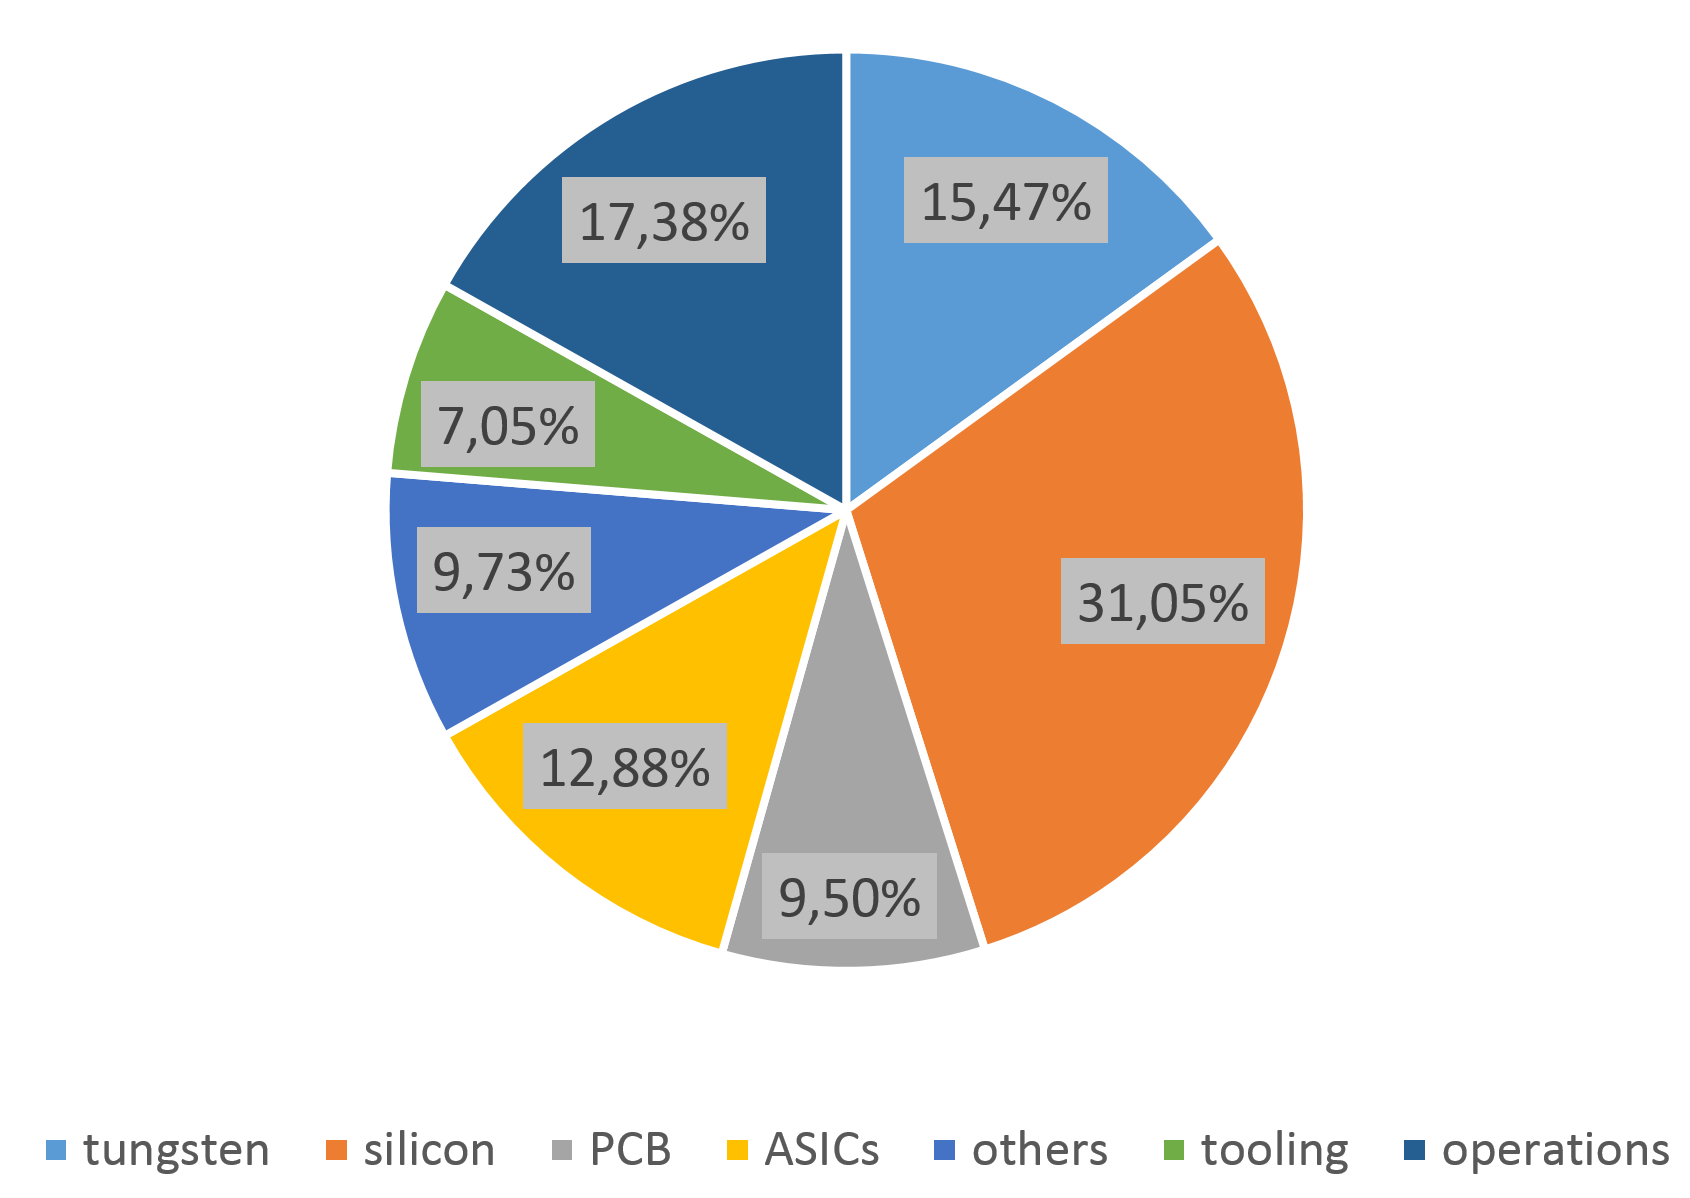
\includegraphics[width=0.8\hsize]{Costing/ECal26_Si_cost_sharing.PNG}
%\caption{Contributions of the different items to the SIECAL cost in the case of the "small model" with a reduced sampling.}
%\textit{The figure should be given for the baseline 30 layers sampling.}}
%\label{fig:det:ECal26_Si_cost_sharing}
%\end{figure}

%\begin{figure}[h!]
%\centering
%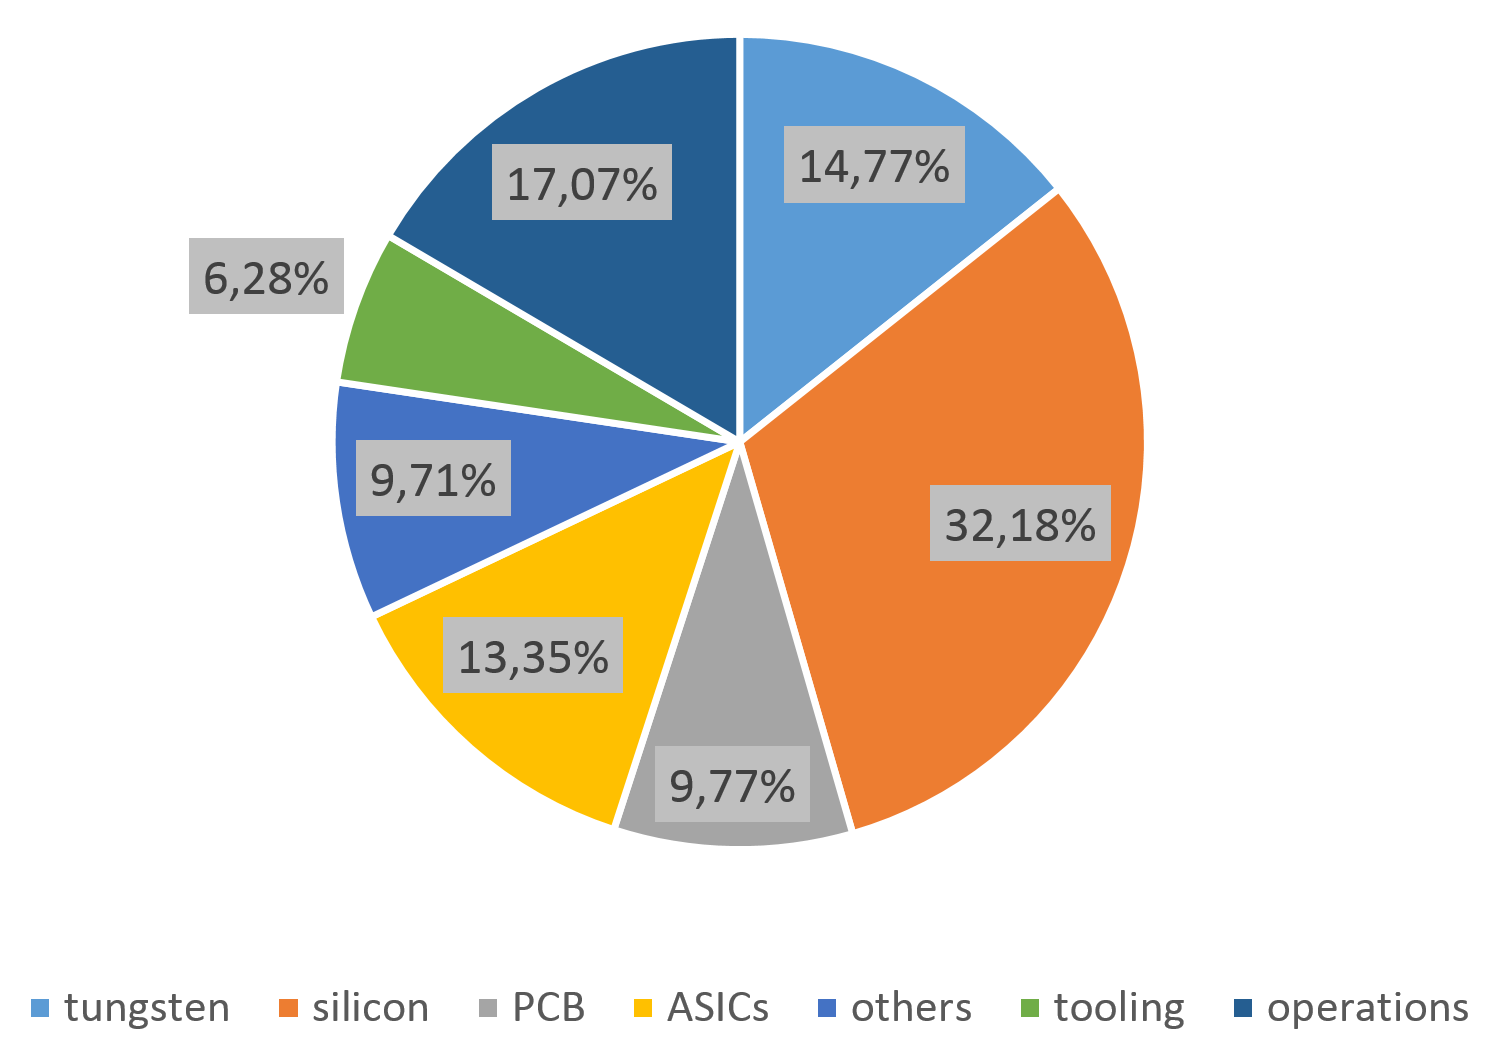
\includegraphics[width=0.8\hsize]{Costing/ECalsm_Si_cost_sharing.PNG}
%\caption{Contributions of the different items to the SIECAL cost in the case of the "small model".} %\textit{The figure should be given for the baseline 30 layers sampling.}}
%\label{fig:det:ECalsm_Si_cost_sharing}
%\end{figure}

\subsubsection{Scintillator version of the ECAL (ScECAL)}
The ScECAL material costing from the DBD is considered to be still valid and corresponds to 74 M\texteuro(2018) for the IDR-L version. The in-house assembly manpower has since then been estimated to 11.5 M\texteuro. Applying simple scaling laws the ScECAL IDR-S version is costed to (62.5, 9.5) M\texteuro.

\subsection{HCAL}

\subsubsection{Analog option (AHCAL)}
Since the DBD the application of the SiPM-on-tile technology to the CMS endcap calorimeter upgrade allows to consolidate the costing further. With about 400000 channels the CMS HGCAL represents an intermediate scale between the 22000 channel AHCAL prototype and the ILD full AHCAL. 
The cost envelopes for the CMS SiPMs are consistent with the scaling assumed for ILD at the DBD times and so far confirmed in informal contacts with vendors. The AHCAL material costing from the DBD is therefore considered to be still valid. It amounts to 44.9 M\texteuro(2018) for the IDR-L version. 
For the IDR-S model, a simple scaling corresponds to a factor 0.84 with a resulting material cost of 37.7 M\texteuro.

No detailed manpower cost estimate has been done. Assuming the same manpower/material ratio as for the SiECAL (9\%) the in-house assembly manpower is estimated to 4 M\texteuro~ for the IDR-L model and 3.4 M\texteuro~ for the IDR-S model.

\subsubsection{Semi-digital option (SDHCAL)}

The SDHCAL material costing from the DBD is considered to be still valid and corresponds to 44.8 M\texteuro(2018) for the IDR-L version. Applying simple scaling laws the SDHCAL IDR-S version is costed to 37.6 M\texteuro~ for material.

No detailed manpower cost estimate has been done. Assuming the same manpower/material ratio as for the SiECAL (9\%) the in-house assembly manpower is estimated to 4 M\texteuro~ for the IDR-L model and 3.4 M\texteuro~ for the IDR-S model.

Note: since the costs for the AHCAL and SDHCAL options are very close to each other they will no longer be distinguished in the HCAL contribution to the global ILD costing.

\subsection{Magnet}
The costing of the magnet (coil and yoke) has been fully revisited. As for the DBD the anti-DID option (section 6.4) is not taken into account since its configuration is not fully defined. The main source of the current evaluation consists of the documentation of the CMS magnet, which has a similar size as that of ILD. When extrapolating to ILD the CHF costs from CMS have been converted into Euros at the exchange parity of the CMS magnet construction time, and the manufactured products price evolution in Europe to 2018 taken into account. The resulting costs are summarised in table~\ref{magnet_cost}. One important change compared to the DBD estimation is the strong reduction in the yoke cost. At the time of the DBD, an iron price of 6ILCU/kg had been agreed upon with SiD and CLIC, whereas the price payed for CMS corresponds to 3.5 \texteuro(2018)/kg. 
In summary the magnet system cost is estimated to (88.5, 9.4) $\approx$ 98 M\texteuro.

No attempt to cost the IDR-S option has been made. A priori the cost of the small version is expected to be reduced. However the impact of the higher nominal field of 4T on the coil winding and on the flux return is not trivial and may counteract the reduced sizes. Keeping the small magnet cost similar to the large one may be a good approximation for the time being.

The magnet costing is likely to still evolve significantly in the future. For the coil, industrial offers are expected from the Japanese companies which are currently studying it, including the anti-DID option. For the yoke, updated designs may significantly reduce the cost, by up to 50\%, as discussed in section 6.4. The yoke final cost will strongly depend on the final stray field constraints retained for ILD, as well as on the evolution of the iron market prices until ILD construction.

%\textit{Check iron cost used in chapter 6.4 to estimate yoke cost reductions given there for various options.}

\begin{table}\hspace*{-0cm}\small 
\begin{tabular}[h!]{ l p{0.2\hsize}  p{0.1\hsize} }
\toprule
%\multicolumn{7}{ l }{{\bf Silicon Inner Tracking}}\\
\textbf{Magnet system} & \textbf{88.5}\\
\midrule
\textbf{Coil} & \textbf{28.5}\\
\midrule
Conductor and winding & 22\\
Internal cryogenics and suspension &  0.2\\
Suspension system & 0.3 \\
%Internal instrumentation & 0.9 \\
Tooling, assembling & 5.4 \\
Qualification and partial testing & 0.6\\
\midrule
\textbf{Ancillaries for coil} & \textbf{11.5}\\
\midrule
Cryogenics and vacuum & 6.5\\
Electrical power circuits & 0.9\\
Control and safety systems& 1.4 \\
Engineering (transport to cavern) & 2.1\\
Integration in cavern& 0.3 \\
Field mapping&0.3\\
\midrule
\textbf{Yoke and vacuum tank} & \textbf{48.5}\\
\midrule
Yoke steel including works and vacuum tank& 39.6\\
Support &1.2\\
Moving system& 2.6\\
Assembly& 4.8\\
Photogrammetry and survey& 0.3 \\
\bottomrule
\end{tabular}
\caption{\label{magnet_cost}Elements of cost of the magnet system in M\texteuro.}
\end{table}

%\begin{figure}[h!]
%\centering
%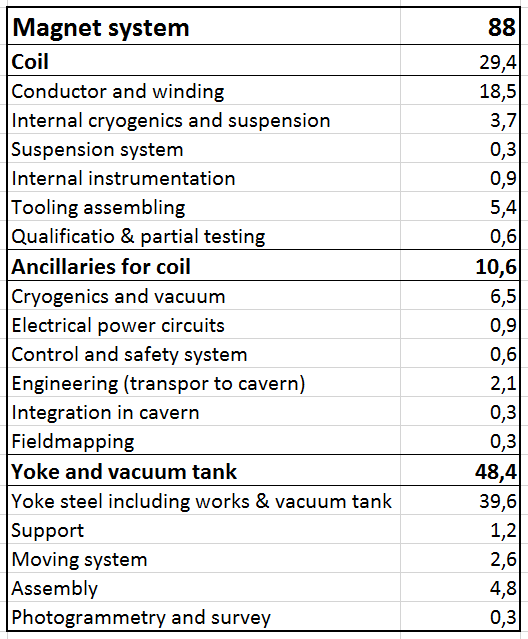
\includegraphics[width=0.5\hsize]{Detector/fig/Magnet_table.PNG}
%\caption{Magnet cost sharing. The costs are in MEuros}
%\label{fig:det:Magnet_cost_sharing}
%\end{figure}


\subsection{Iron yoke instrumentation}
There is no update since the DBD, where the quoted iron instrumentation material cost corresponded to 6.5 M\texteuro(2018) for instrumentation of the 14 layers of the large IDR-L version. Using simple scaling laws the Iron instrumentation of the IDR-S option is estimated to 6.0 M\texteuro.

%\textit{For how many instrumented layers ?}

No assembly tooling and manpower has been estimated. Based on the SiECAL detector these contributions can be estimated to 0.6 M\texteuro~ for both the large and small options. 

\section{Global ILD costing.}
The subdetector costs are summarised in table~\ref{cost_summary} for their baseline design. The two ILD models IDR-L and IDR-S are considered separately and global sums computed using the SiECAL option for the ECAL.
The inner system which offers no difference between the two sizes sums up to 22.7 + 4.9 = 27.6 M\texteuro. The outer system sums up to 319.1 + 32.0 = 351.1 M\texteuro~ for IDR-L and 274.2 + 27.1 = 301.3 M\texteuro~ for IDR-S.
The item labelled "global" includes the central DAQ, integration and transportation. These contributions have not been revisited since the DBD and have some overlap with items in the subdetector sections. Their total amount is directly reproduced from the DBD.
%\textit{Add comment on global components (DAQ, etc...)}

\begin{table}[h!]\hspace*{-0cm}\small
\begin{tabular}{ l p{0.15\hsize}p{0.15\hsize}p{0.15\hsize} p{0.15\hsize}p{0.15\hsize}}
\toprule
\bf {ILD COSTING (M\texteuro~ 2018)}& \bf {IDR-L} & \bf              &  \bf {IDR-S}&\bf \\
\bf {Item}      & \bf material & \bf manpower &  \bf material &\bf manpower \\
\midrule
Beam tube& \it0.5 &  \it0.& idem&idem \\
VTX        & 2.96  &1.45  &  idem &idem \\
SIT        & 5.0   &1.5 & idem&idem\\
%SIT pixels & 7.55  &2.0 & idem&idem\\
FTD       & 4.8   &1.3  & idem &idem  \\
%FTD pixels  & 6.3  &1.7  & idem &idem  \\
LumiCAL & 3.37  & 0.16& idem&idem\\
ECAL ring & 1.5 & 0.16 & idem&idem\\
LHCAL   & 2.93  & 0.16&idem& idem\\
BeamCAL & 2.15  & 0.16& idem&idem\\
%FCAL    & 9.95  & 0.64& idem&idem\\
\bf{Inner part total} &\bf{23.2}&\bf{4.9}&\bf{idem}&\bf{idem}\\
%Inner part new    &32.8&7.4&idem&idem\\
\midrule
TPC & 25.2 & 5 & 19 & 3.6\\
%SET & 12.6& 1.9&10.8&1.7\\
SET    & 20& 2&16&1.5\\
SiECAL & 119 & 11.0 & 92. & 8.7\\
ScECAL & \it74 & 11.5 & \it62.5 & 9.5\\
AHCAL  & \it44.9 & 4 & \it37.7 & 3.4\\
SDHCAL & \it44.8 & 4 & \it37.6 & 3.4\\
Coil and ancillaries &  40 & 4& idem & idem\\
Yoke and vacuum tank &  48.5 & 5.4& idem & idem \\
Iron instrumentation  &  \it6.5 & 0.6 & 6 & 0.54\\
\bf{Outer part total}&\bf{304.1}&\bf{32.0}&\bf{259.2}&\bf{27.1}\\
\midrule
%DAQ           & \it1.1 & \it0.16& idem& idem\\
%Integration   & \it1.5 & \it0   & idem& idem\\ 
%Transportation& \it12  & \it0   & idem & idem \\
\bf{Global (DAQ, integration, transport)}  &\bf{\it14.6} &\bf{\it0.16}& \bf{idem}& \bf{idem}\\
\midrule
\bf{Total} & \bf{342}   &  \bf{37.0}  & \bf{297.0} & \bf{32.2}  \\
%New version       & 351.6   &  39.0  & 306.6 & 34.3  \\
\midrule
\bf{Grand Total including manpower}    & \bf{379}   &    & \bf{329} &   \\
%Total including MP new     & 392   &    & 341 &   \\
 \bottomrule
\end{tabular}
\caption{\label{cost_summary}Global cost estimate of ILD in its baseline design (M\texteuro~ 2018). The numbers in italic are extrapolated from the DBD. The manpower has been translated from FTExYears to Euros. The total sums are computed with the SiECAL option.
}
\end{table}
Table ~\ref{cost_summary} presents only the costing of the IDR-L and IDR-S baseline design. Some variants such as fully pixelised inner detectors, reduced sampling in the SiECAL or reduced return yoke have been discussed and costed above. Their individual impacts on the cost of the small IDR-S ILD version are summarised in table ~\ref{cost_variants}, together with the result of taking all of them into account.
%\textit{Add table showing IDR-S global cost variations with various possible changes: pixels in SIT/FTD, Yoke, reduced ECAL sampling ...}
\begin{table}[h!]\hspace*{-0cm}\small
%\begin{tabular}{ l p{0.15\hsize}p{0.15\hsize}p{0.15\hsize} p{0.15\hsize}}
\begin{tabular}{ccccc}
\toprule
\bf {Baseline design} & \bf Fully pixelized inner trackers &  \bf Reduced ECAL sampling&\bf Reduced yoke&\bf Altogether\\
\midrule
329&337&318&320&316\\
\bottomrule
\end{tabular}
\caption{\label{cost_variants}IDR-S costing taking into account several variants discussed in the text, individually and altogether, in M\texteuro.}
\end{table}

\section{Comparison to the DBD cost estimate and discussion.}
 
 The DBD ILD total cost corresponded to 392 M\texteuro(2018), with a relative sharing between subdetectors shown on Figure~\ref{fig:det:DBD_cost_sharing} left. The same figure shows on the right the sharing for IDR-L.
 
 The updated cost sharing for IDR-S is shown on Figure \ref{Costing:Small_cost_sharing} left. As an illustration of the potential effect of design changes the cost sharing is also shown on Figure \ref{Costing:Small_cost_sharing} right for ILD-S with SIT and FTD totally equipped with pixels, and sampling reduced to 26 layers in the SiECAL.
 
\begin{figure}[h!]
\begin{tabular}{cc}
%\centering
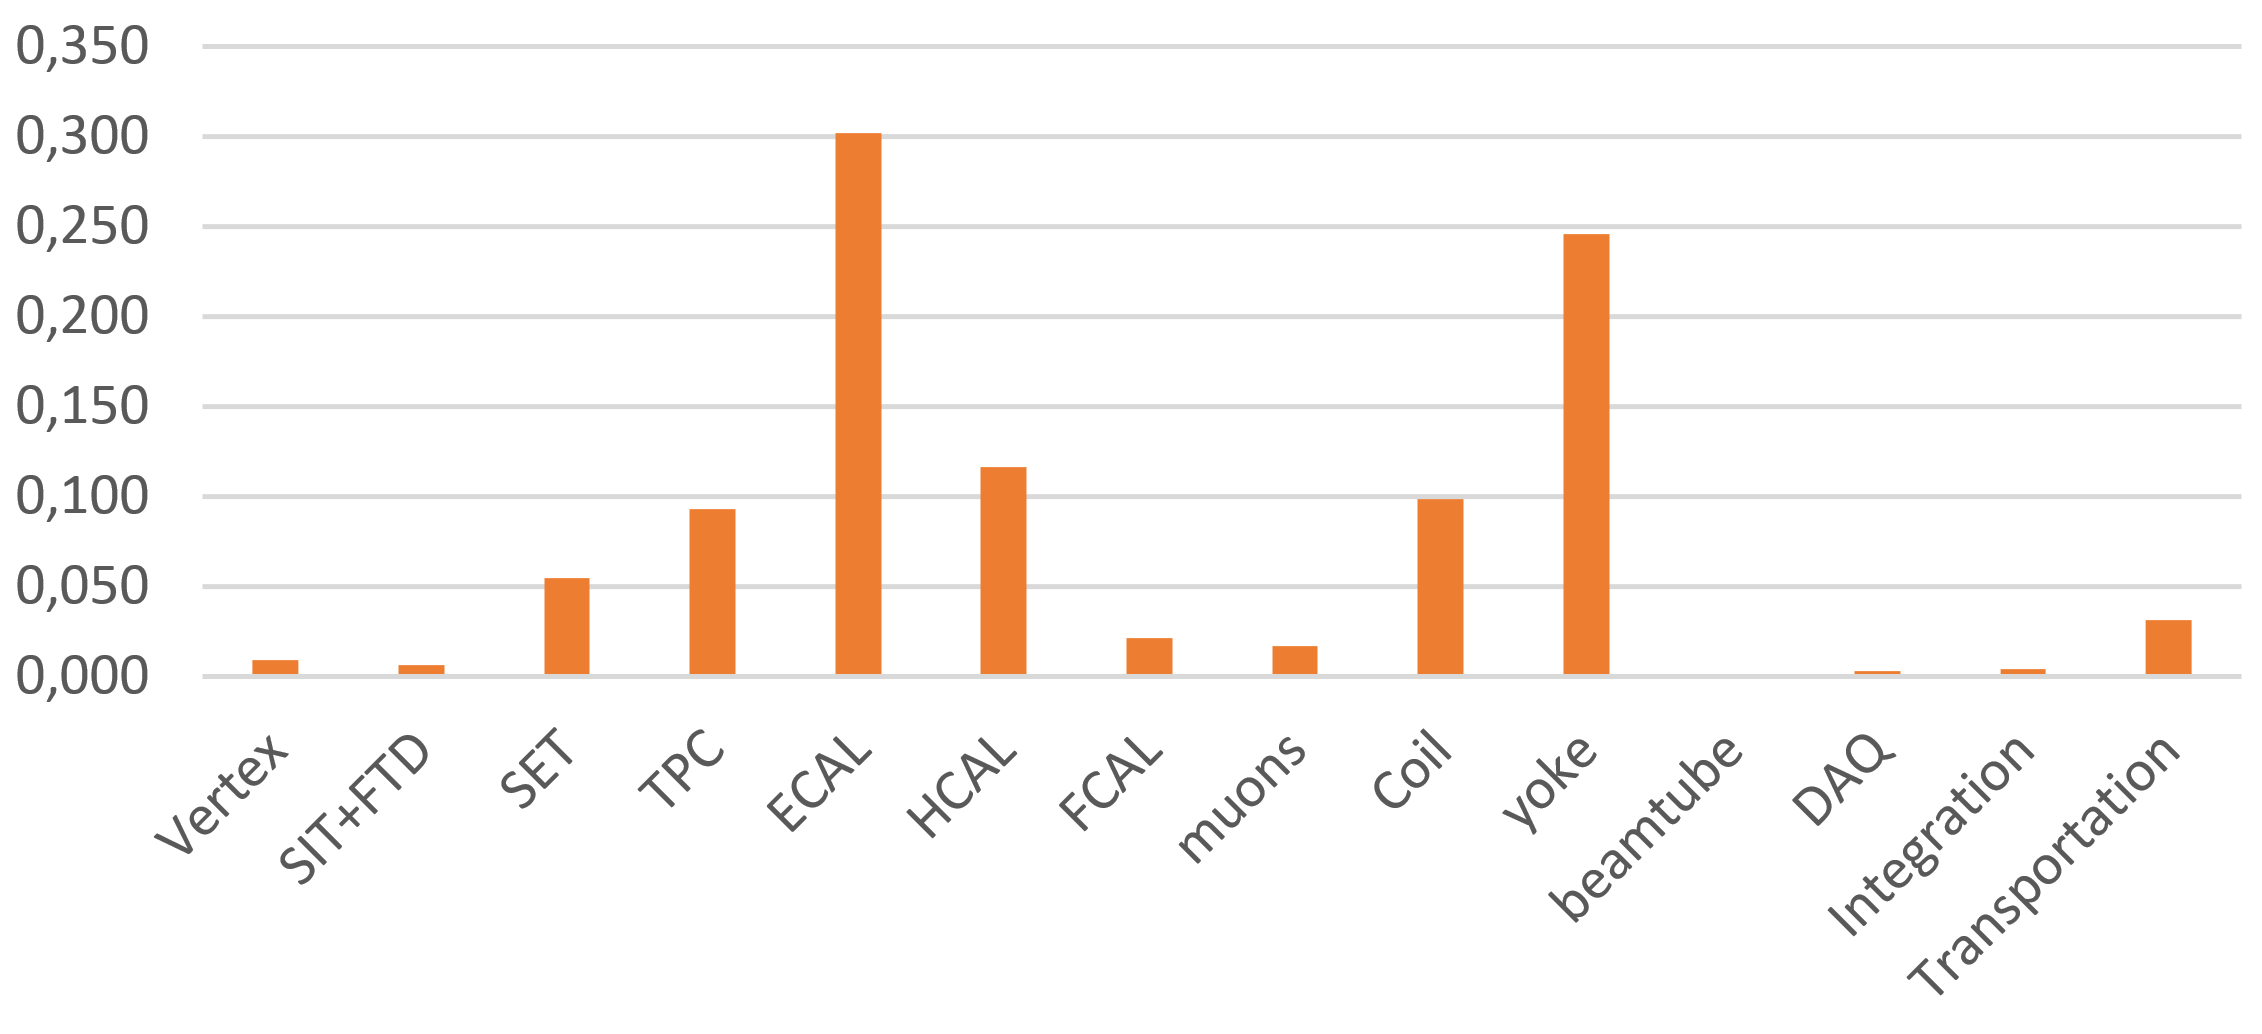
\includegraphics[width=0.47\hsize]{Costing/DBD_cost_sharing.PNG}&
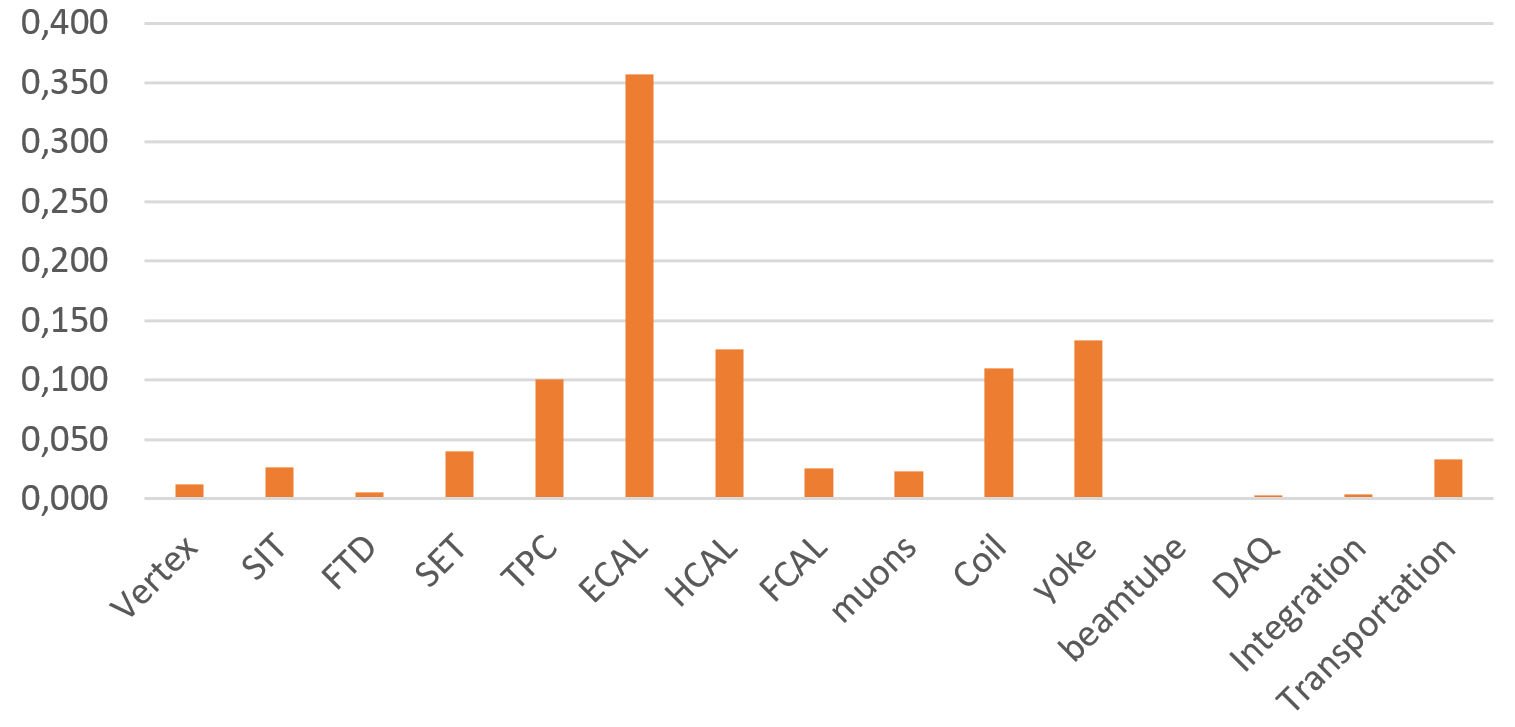
\includegraphics[width=0.47\hsize]{Costing/Large_cost_sharing.PNG}
\caption{ILD cost sharing as documented in the DBD (left), and for the large IDR-L version (right)}
\label{fig:det:DBD_cost_sharing}
\end{tabular}
\end{figure}

%\begin{figure}[h!]
%\centering
%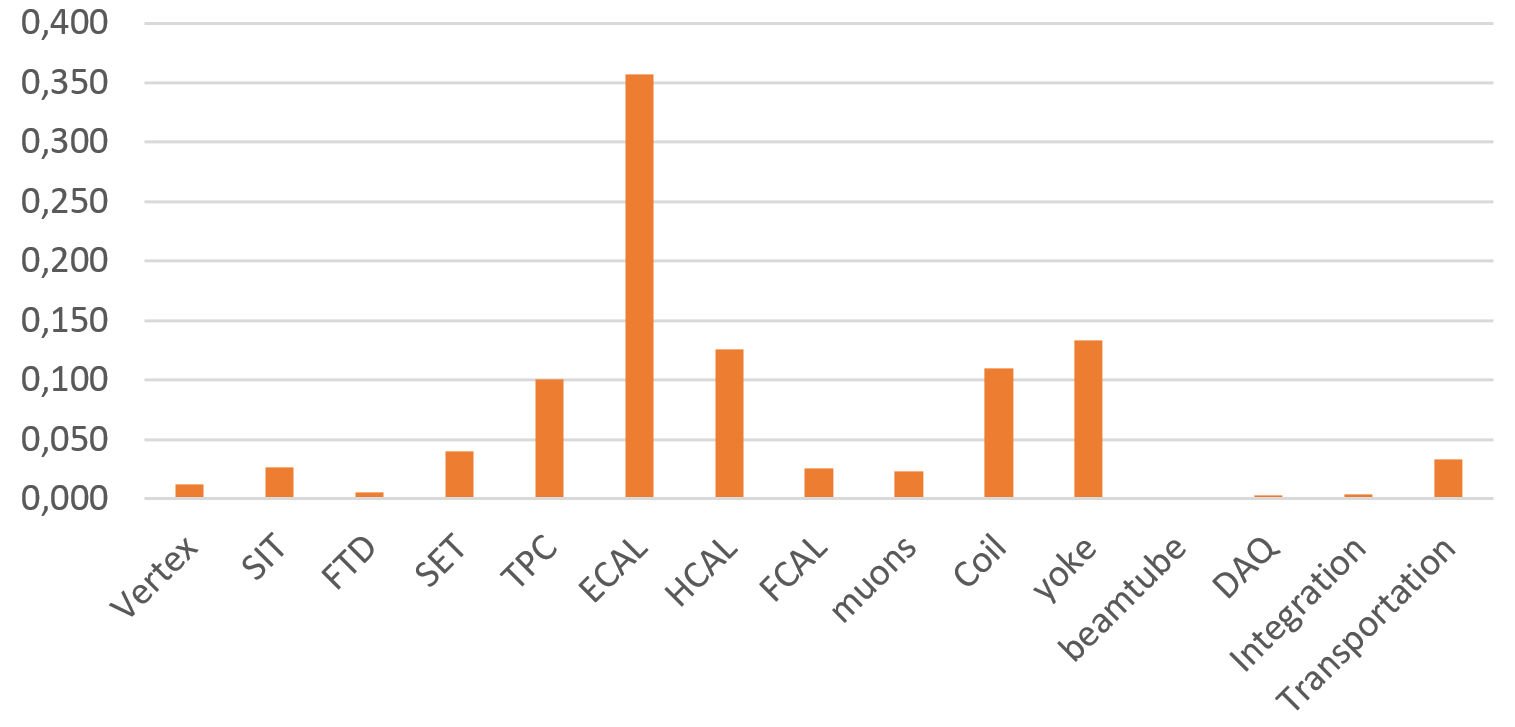
\includegraphics[width=0.6\hsize]{Costing/Large_cost_sharing.PNG}
%\caption{ILD cost sharing for IDR-L baseline design. }
%\label{Costing:Large_cost_sharing}
%\end{figure}

\begin{figure}[h!]
%\centering
\begin{tabular}{cc}
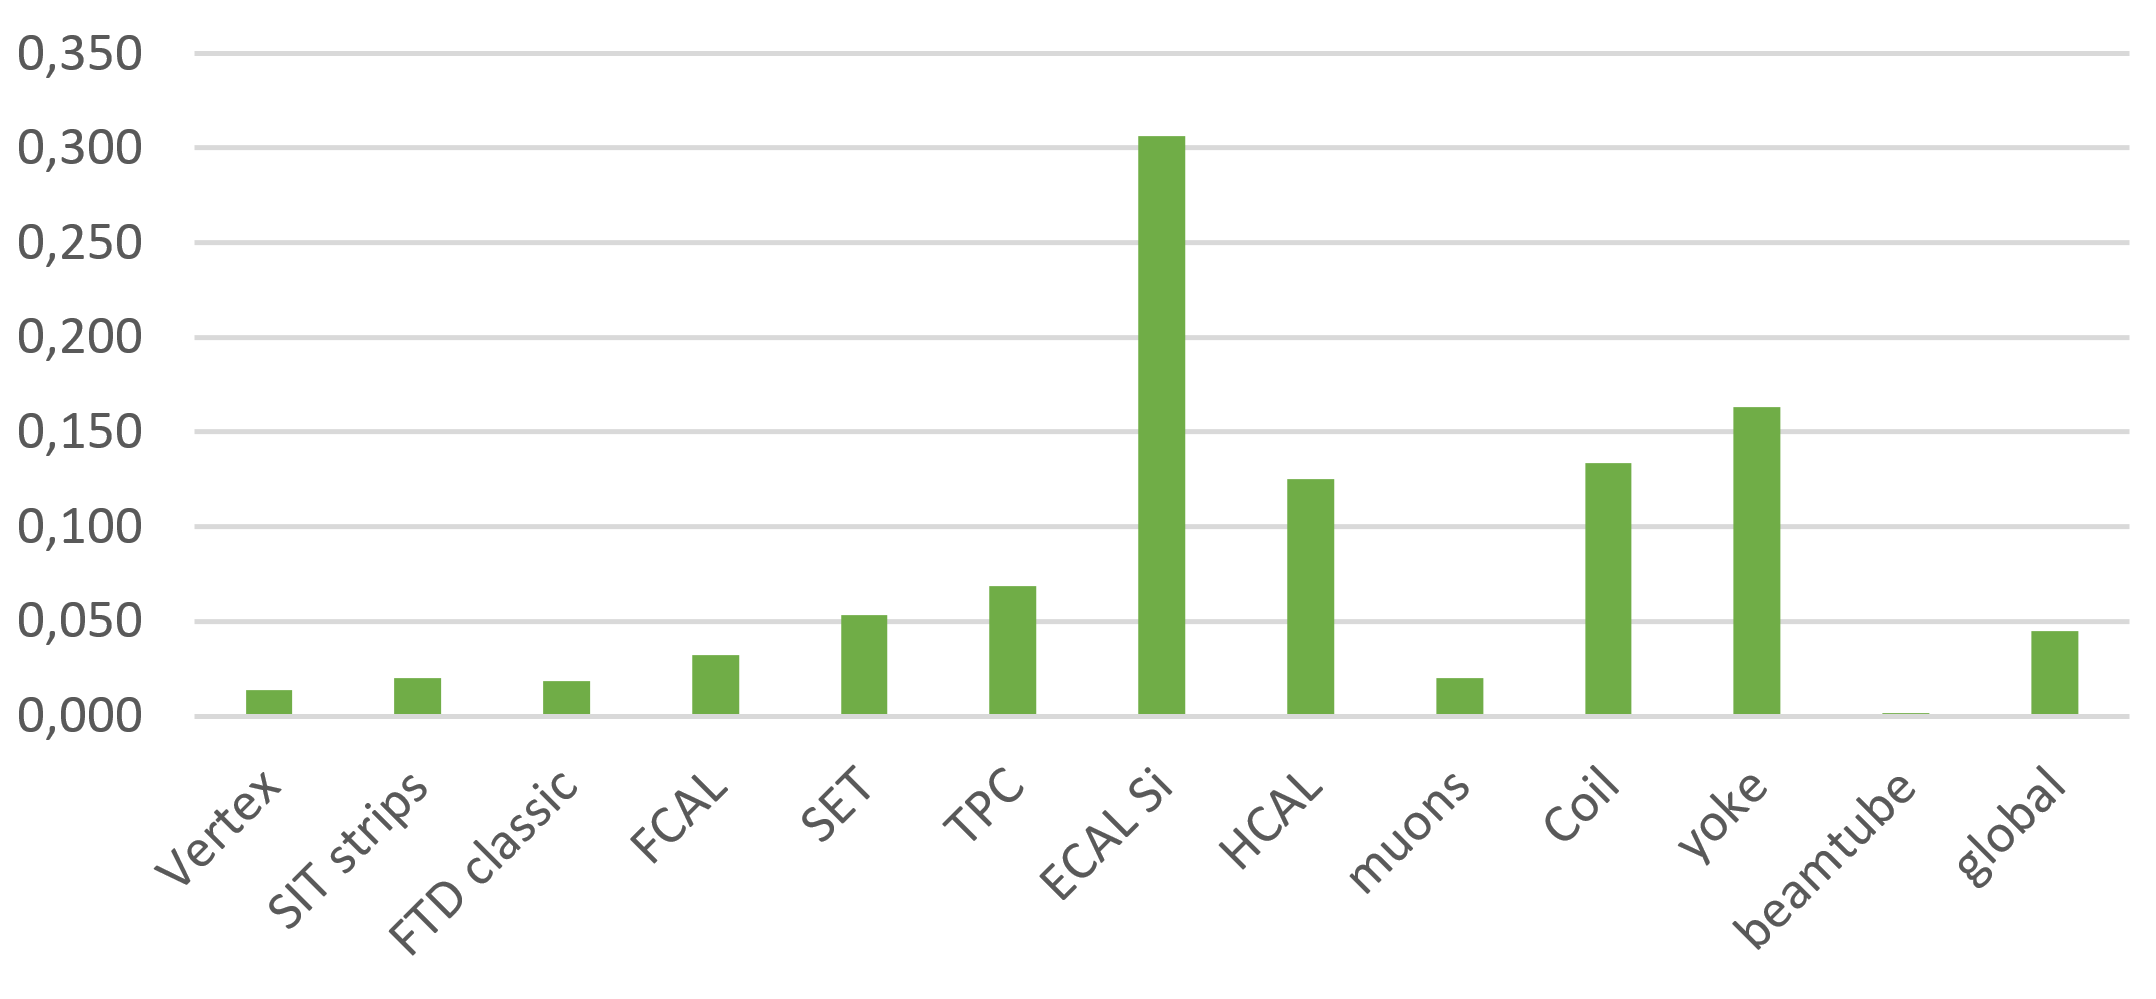
\includegraphics[width=0.47\hsize]{Costing/Small_cost_sharing.PNG}&
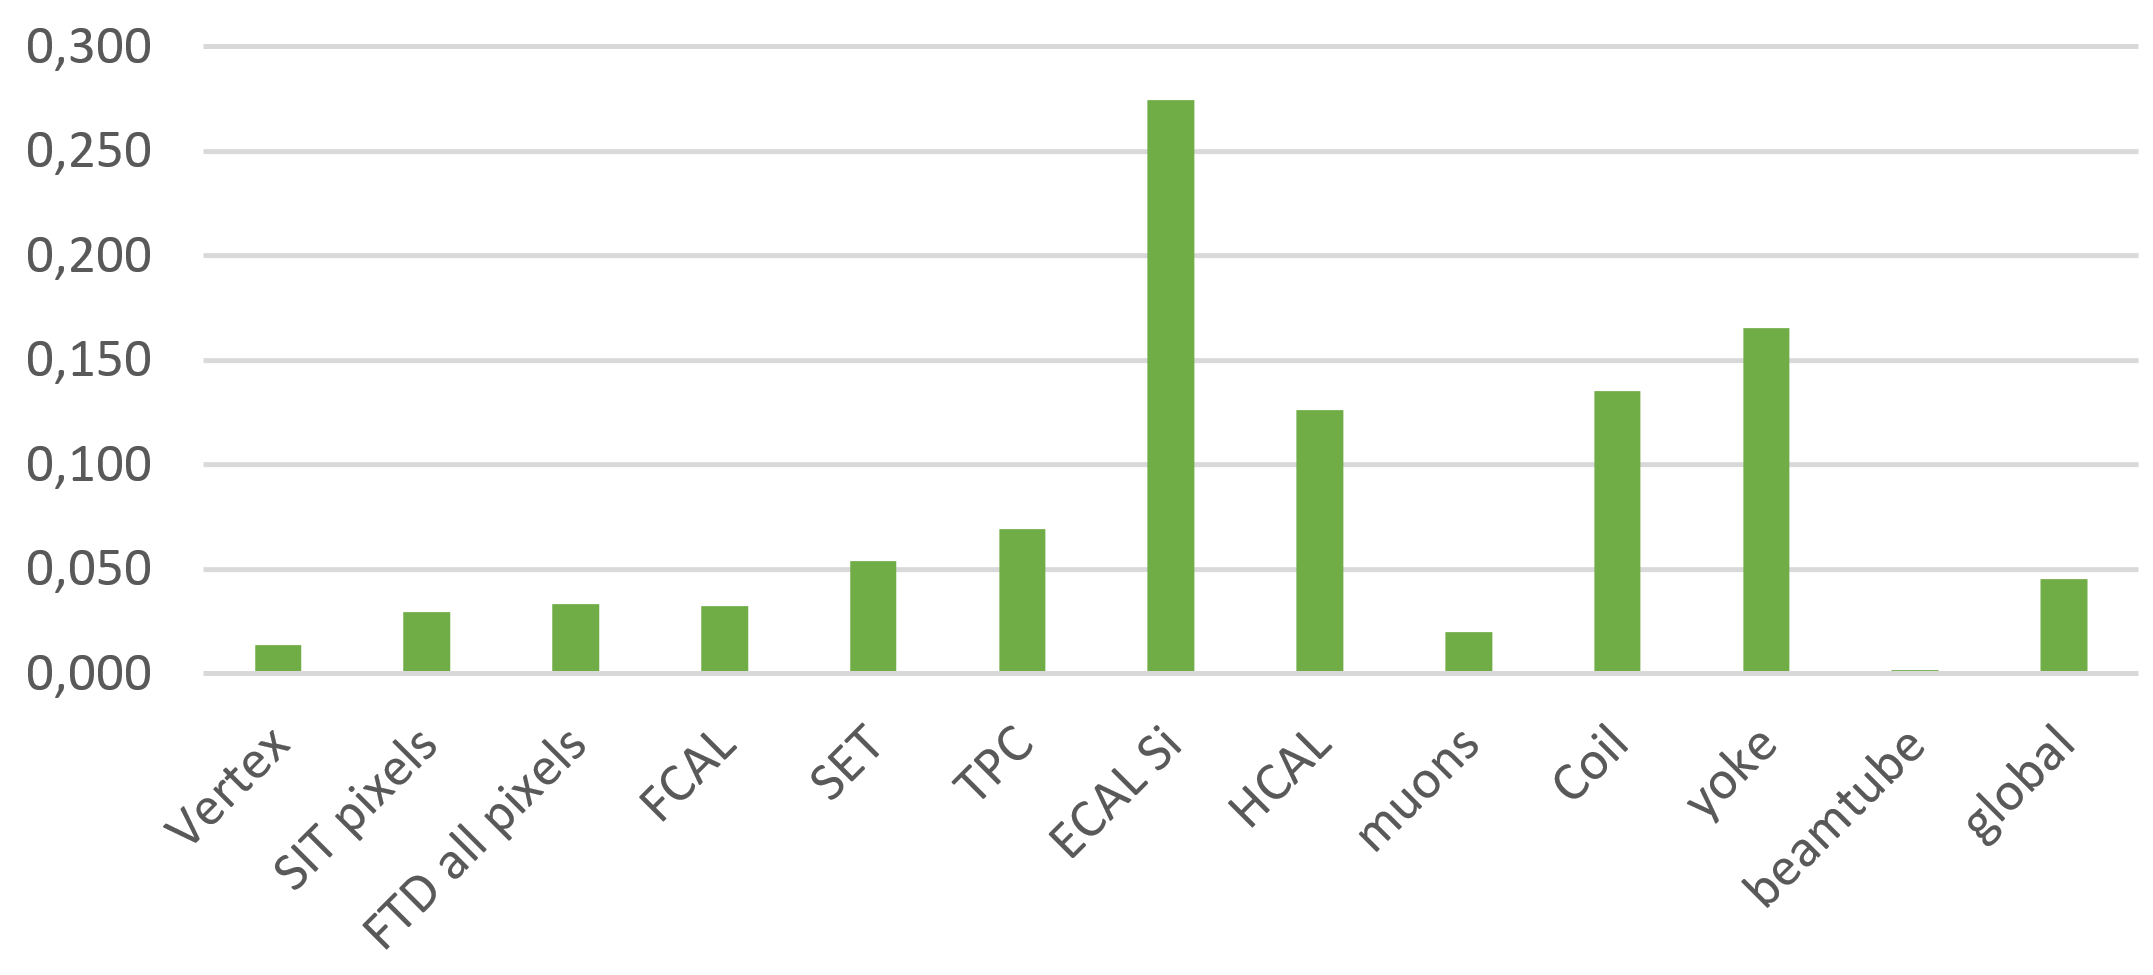
\includegraphics[width=0.47\hsize]{Costing/Small26_cost_sharing.PNG}
\caption{ILD cost sharing for the IDR-S small version in its baseline design (left), and modified with full pixel inner tracking and SiECAL reduced sampling for a total cost of 326M\texteuro~ (right). }
\label{Costing:Small_cost_sharing}
\end{tabular}
\end{figure}

%\begin{figure}[h!]
%\centering
%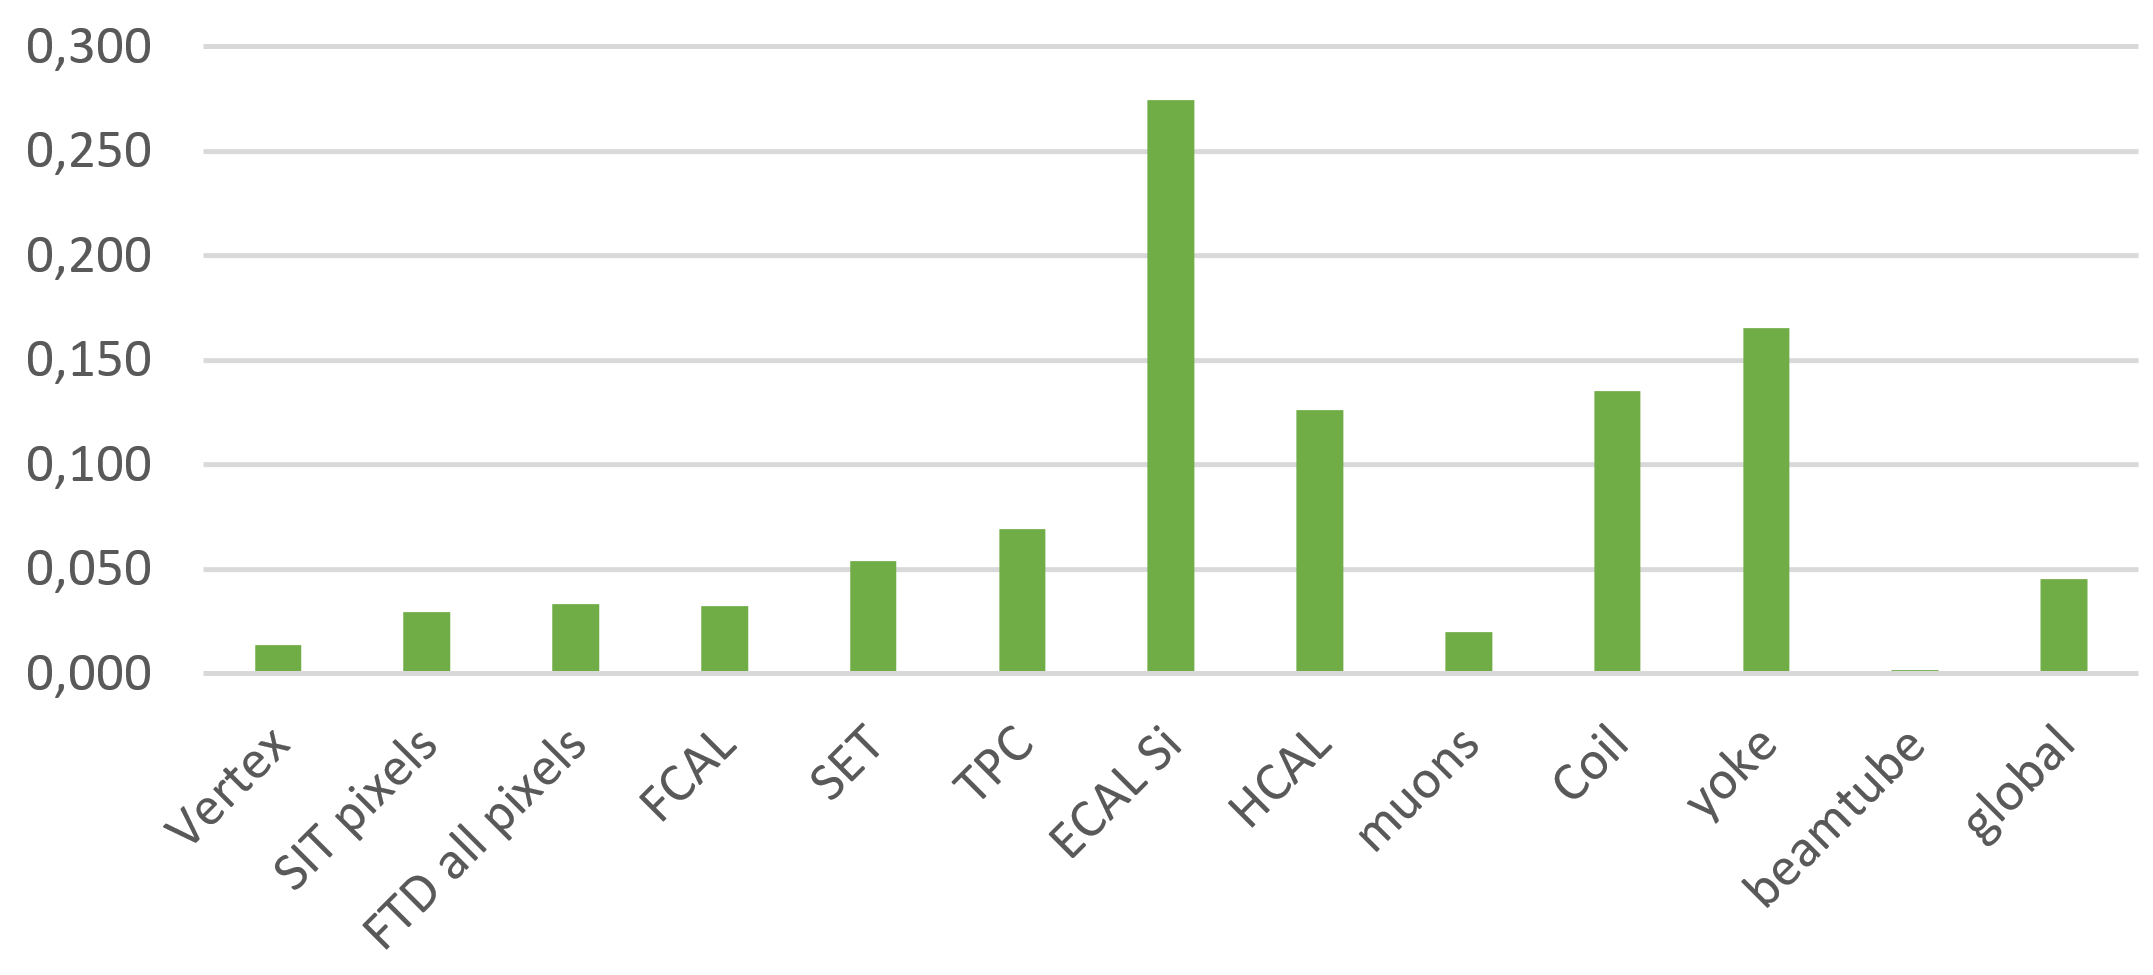
\includegraphics[width=0.6\hsize]{Costing/Small26_cost_sharing.PNG}
%\caption{ILD cost sharing for IDR-S upgraded with full pixel inner tracking and SiECAL sampling reduced to 26 layers (total cost of 330MEuros). }
%\label{Costing:Small26_cost_sharing}
%\end{figure}

When comparing the updated estimations to the DBD one, it should be reminded that the latter did not include in house manpower in most cases, and that the DBD ECAL was a mix of the Silicon and Scintillator options. 
One important message of the new estimation is that the dominant SiECAL contribution has reduced significantly using latest information from the ongoing spin-off projects of the technology, and that further reduction could be achieved by reducing the sampling. In the same vein the yoke cost, which has been kept identical for the two options, could be reduced by a significant amount depending on its design and the stray field which can be accepted. 

The size reduction of IDR-S provides a saving of about 50M\texteuro~ compared to IDR-L. This $\approx$15\% cost reduction will have to be considered in regards with the performance comparison of the two size options.

In summary, the ILD technology maturation since the DBD times has comforted the global detector cost estimation in the direction of lower costs. New detection features w.r.t the current baseline design, such as enhanced pixel tracking and high resolution timing, may increase the costs in the future. However several options for further cost reduction have been identified and require further studies to assess their impact. 

